\chapter{Two-frequency Cognitive Radio Test-Bed}
The main aim of this project is to demonstrate the coexistence of 
primary users and secondary users in the GSM band. Also it has to be
ensured that primary users is given a higher priority over the 
secondary users and there should be no mutual interference. Analysis 
of radio spectrum assigned to primary users conclude that it is most of the time underutilized. 
The spectrum bands which are assigned to primary user and are not utilized by
them at certain time instants are called spectrum holes. 
So in order to accomplish coexistance of primary and secondary users, 
implementation of a cognitive radio which detects these spectrum holes in the 
radio spectrum and enables secondary users to utilize these for communication 
is needed. An experimental setup is developed for this demonstration using 
OpenBTS and GNU radio software and USRP N210 as hardware. First a 2-frequency 
system is developed which is then expanded to a 4-frequency system.



\begin{figure}
\centering
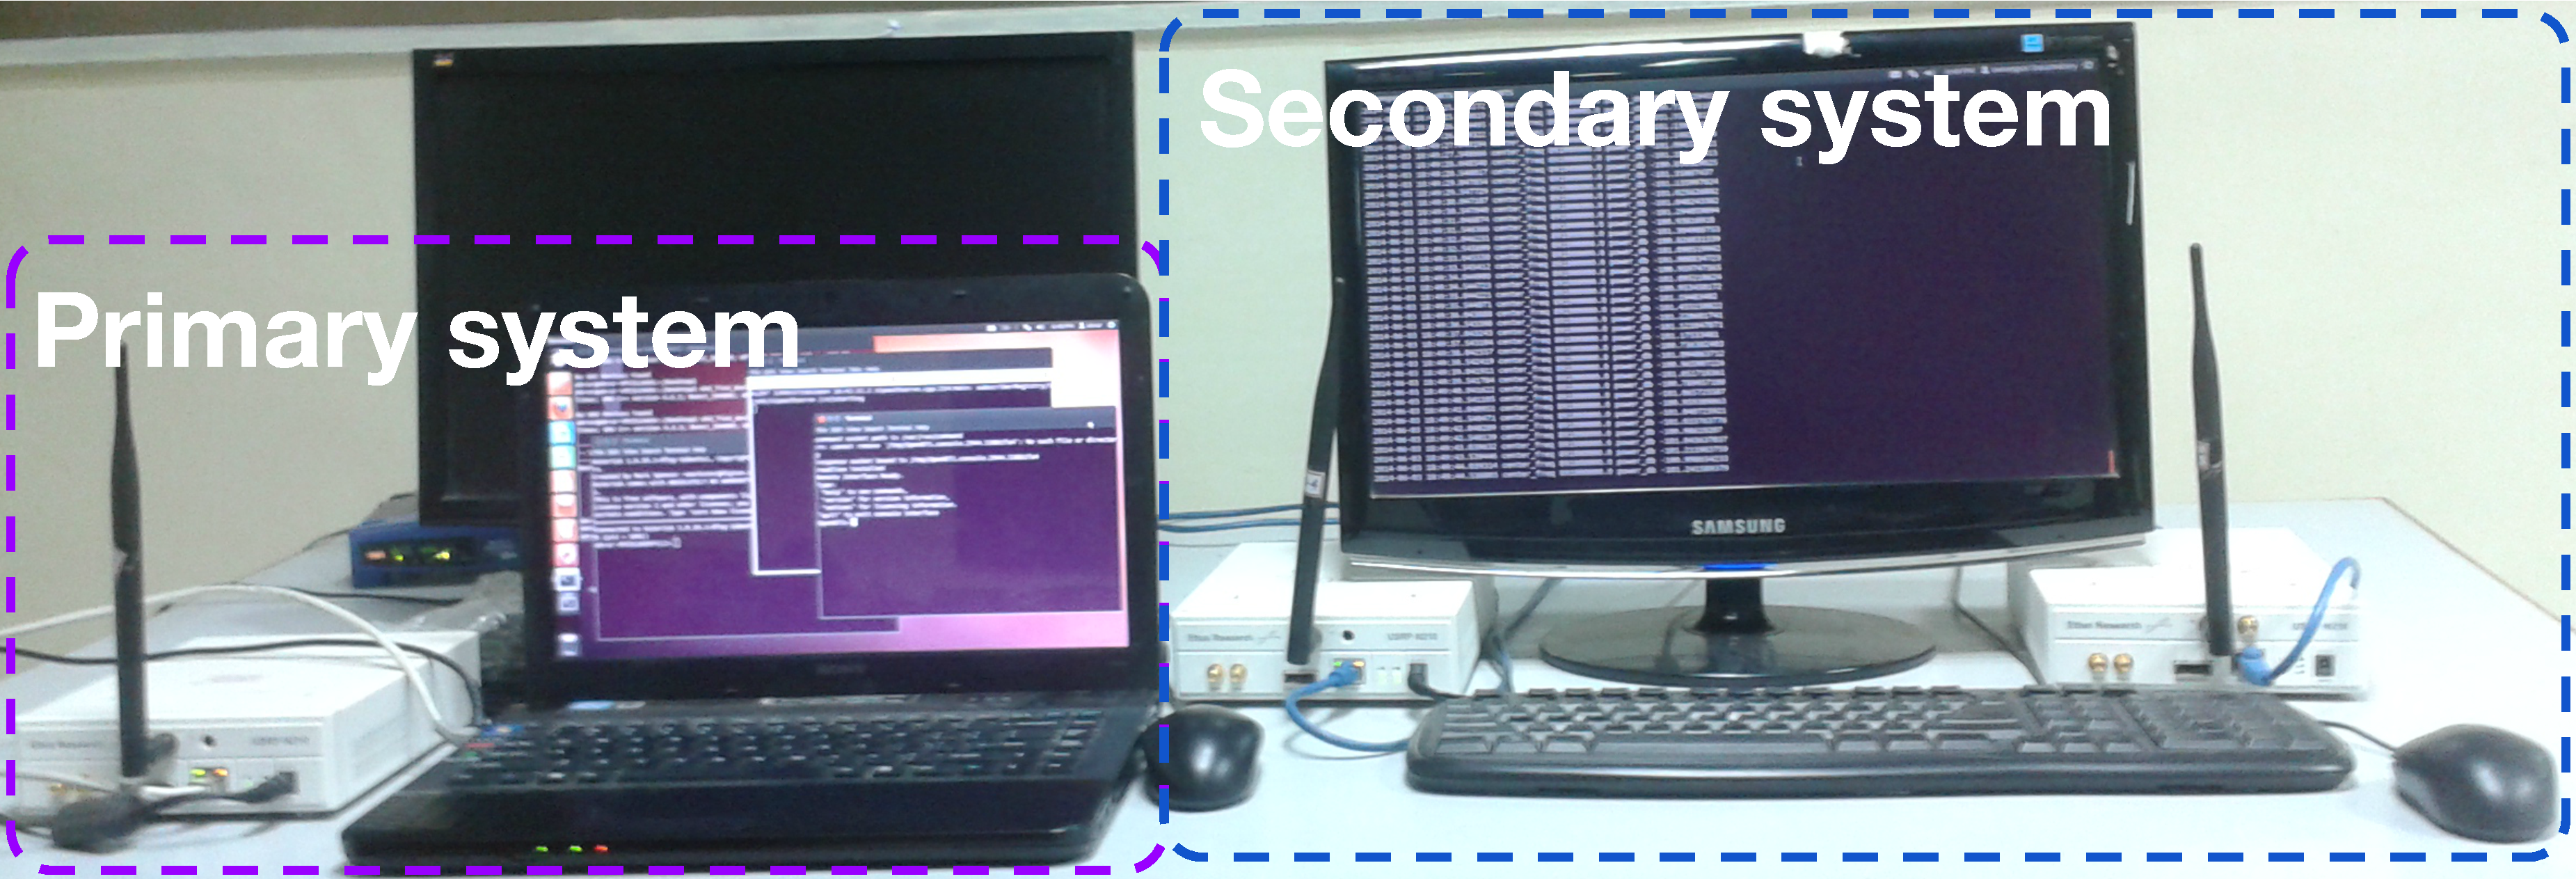
\includegraphics[width=1\textwidth]{../images/freq2}
\caption[Experimental setup, 2-frequency system]{Experimental setup of the 
2-frequency system}
\label{freq2}
\end{figure}


\subsection{2-frequency system description}
Figure \ref{freq2} describes the experimental setup for 2-frequency system. It 
consist of one primary and one secondary subsystems. The primary subsystem has 
only OpenBTS software and one USRP for RF front. Where as secondary subsystem 
has OpenBTS along with GNU radio and two USRP kits for each of these softwares 
as hardware RF front. This secondary subsystem has cognitive capabilities. To 
provide cognitive capabilities it was necessary for OpenBTS and GNU radio to run 
together in the same computer and communicate with each other which was challenging. 
Secondary subsystem continuously senses the frequency band of interest and  
takes decision depending upon the analysis of the data collected and changes 
its parameters accordingly so that primary and secondary users coexist. The 
spectrum sensing is accomplished by using GNU radio.  GNU radio and 
OpenBTS of the secondary subsystem were made to coordinate and behave in appropriate manner and take dynamic decisions 
as and when required to make over all system behave cognitively.

\subsection{2-frequency system testing}
For 2-frequency cognitive system, two GSM bands are used with centre 
frequency 945MHz ($F_1$) and 950MHz ($F_2$). Secondary users are made to occupy 
one of these two bands say $F_1$. Then we make primary users enter the same 
band. This results in an increase in energy levels in this band which is sensed 
by the secondary subsystem as it is continuously scanning this band. 
Immediately secondary users are shifted to other frequency band ($F_2$) thereby 
vacating $F_1$ for primary users. Periodogram analysis is used to calculate the energy levels in the band.
 Hence a 2-frequency cognitive system 
demonstrating coexistence of a pair of primary and secondary users is 
accomplished. 
The whole technique for this cognitive behavour of the secondary subsystemis described using a flow graph shown in figure
\ref{freqSys2}:

\begin{figure}[!h]
\centering
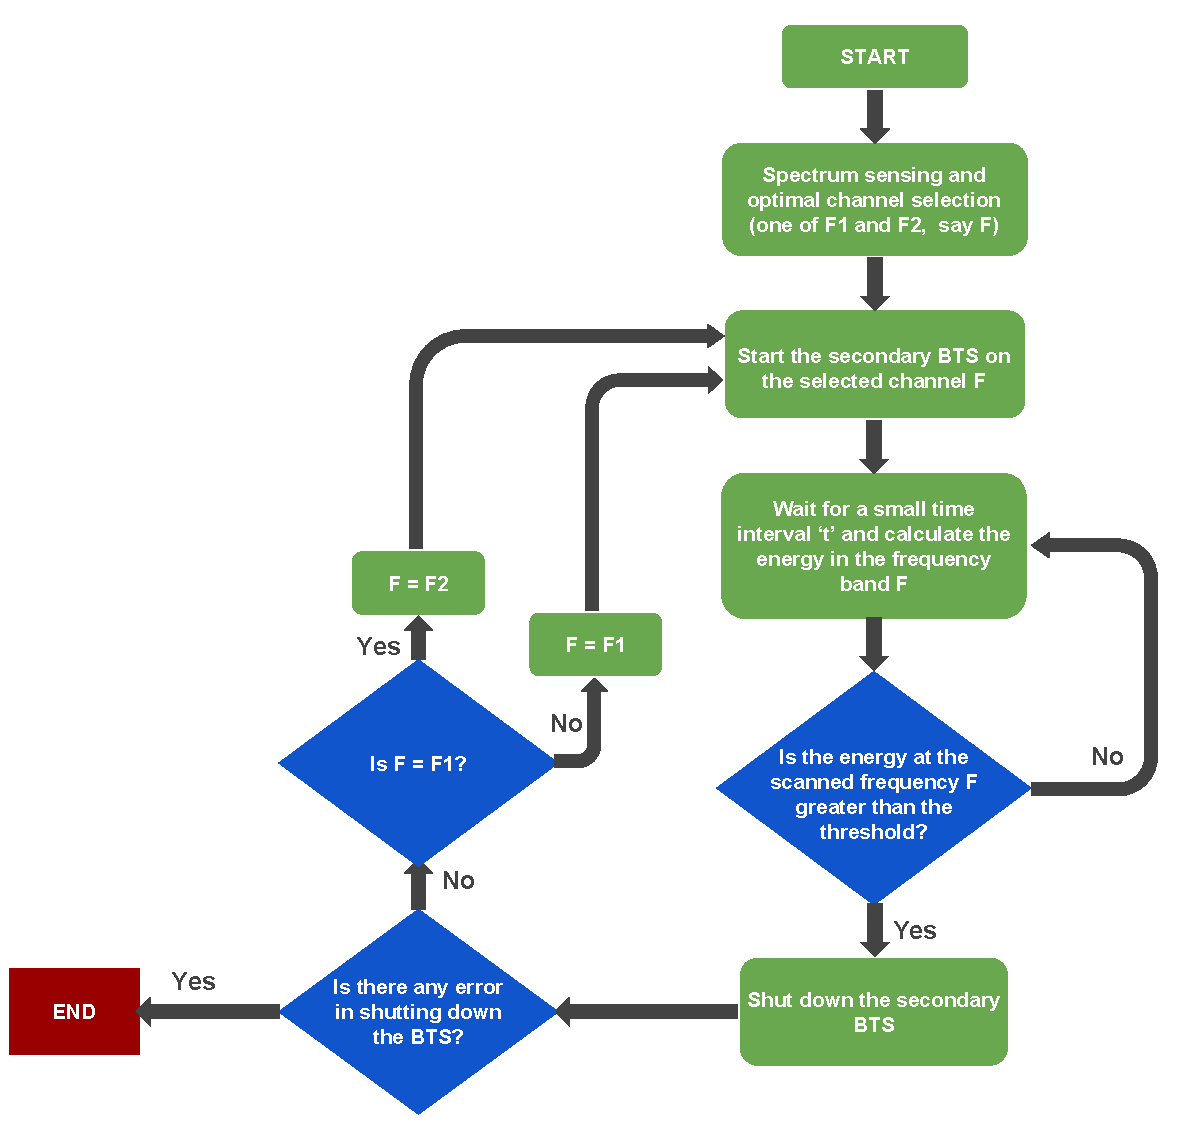
\includegraphics[width=1\textwidth]{../images/freqSys2}
\caption[2-frequency system]{Flowchart for 2-frequency system}
\label{freqSys2}
\end{figure}

As we can see in the flow graph, we begin with spectrum sensing where we choose optimal channel out of 945MHz and 950Mhz for secondary OpenBTS operation.
Then secondary OpenBTS is made to operate on this channel which is utilized for communication by secondary users. 
This band of operation is continously scanned after every time interval 't' to check for the presence of primary radio. If energy is lower than predefined threshold we rescan the channel as it is seen in the flow graph.
If at any time instant the energy is found to be higher than the predefined threshold,
 we conclude that primary radio has appeared and there is a need to vacate the channel. Hence  OpenBTS of the secondary subsystem is switched off and 
restarted with now frequency band of operation as F1 if it was F2 previously and viceversa. And next we go back to the second step in the flow graph that is contious spectrum scanning. 
If there are any issues in switching off of the OpenBTS the algorithm reaches end.





\section{CUSUM}
CUSUM peak detection is also applied after energy detection to ensure that the
detected high energy in the band of interest is not due to some irrelevant 
reasons like random fluctuations in noise power etc, but due to the presence of 
primary radio in that band. This ensures high accuracy in primary radio 
detection and correct decision making.
CUSUM is basically a sequential analysis technique to detect change. 
It is a criterion for deciding when to take corrective action. As the name 
implies CUSUM involves calculating cumulative sum. This makes it sequential. 
The samples from a process $x_n$  are assigned weights $\omega_n$  and summed 
as followed,

\begin{align}
S_0 &= 0; \nonumber \\
S_{n+1} &= max(0, S_n + x_n - \omega_n) \nonumber
\end{align}
When the value of $S$ exceeds a certain threshold value a change in value has 
been found. This formula detects change only in positive direction. To detect 
change in negative direction we have to do min operation instead of max 
operation and the change  is detected when value goes below the threshold.

